\begin{enumerate}
	\item zu normalisernder Vektor= [50, 100,200, 300, 400, 600, 1000, 1100]
	\begin{itemize}
		\item min-max = [0, 0.05, 0.14, 0.24, 0.33, 0.52, 0.9, 1]
		\item zscore = [-1.05, -0.92, -0.67, -0.42, -0.17, 0.33, 1.33, 1.58]
	\end{itemize}
	\item der Person-Koeffizient von 0.8176 zeigt eine starke lineare Abhängigkeit an. Der Fitness-Plot unter Abbildung zeigt dies ebenfalls %TODO 
	\item bin by mean= [[ 43.33, 43.33, 43.33], [55,55,55], [80,80,80], [92.7,92.7,92.7], [153.3, 153.3, 153.3], [190, 190, 190], [225, 225, 225]]

\end{enumerate}

\begin{figure}[p]
	\centering
	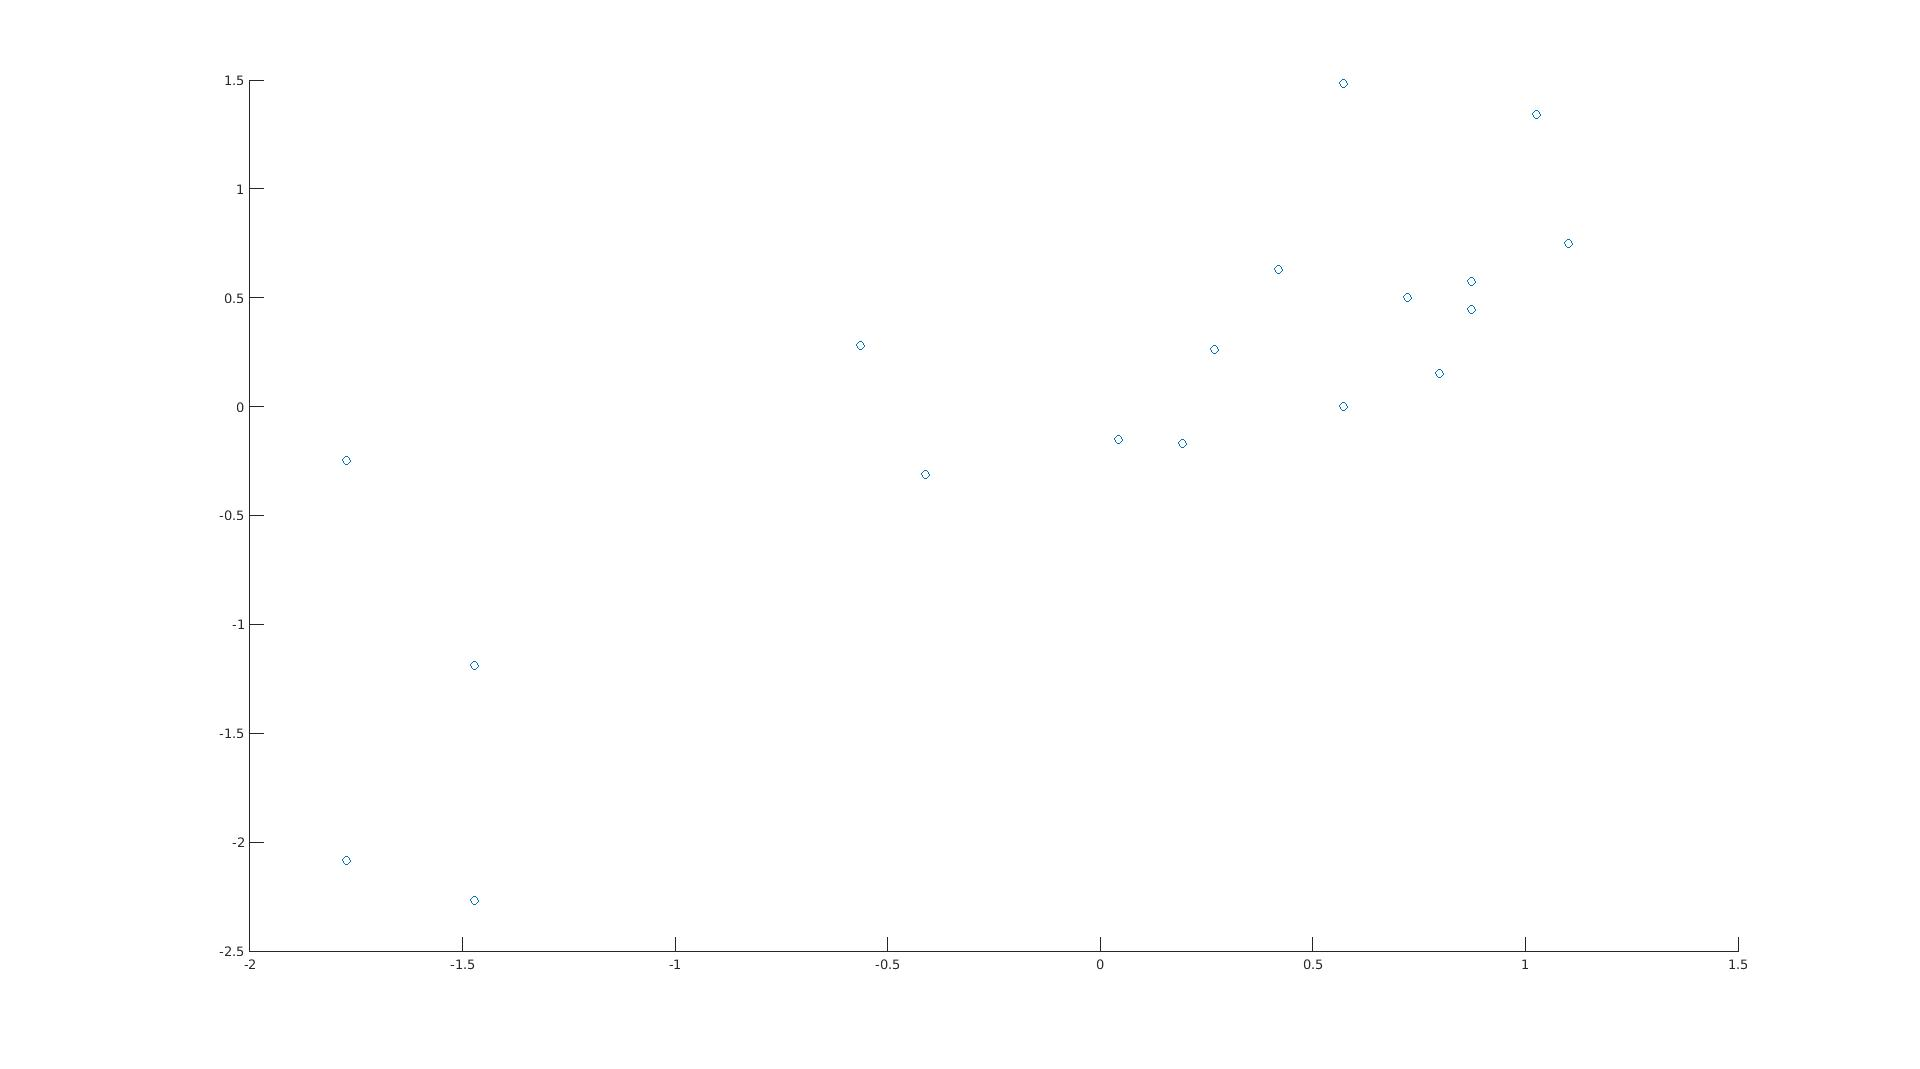
\includegraphics[scale=0.26]{task3_2.jpg}
	\caption{Fitness-Plot}
\end{figure}
